\documentclass[lang=cn,a4paper,newtx]{elegantpaper}

\title{面向多场景泛化的空间先验与时序卷积融合声源定位}
\author{}
\institute{}
\version{}
\date{}

\usepackage{array}
\newcommand{\stft}{\operatorname{STFT}}
\newcommand{\wrap}{\operatorname{wrap}}
\newcommand{\sigmoid}{\operatorname{sigmoid}}
\addbibresource[location=local]{reference.bib}

\begin{document}

\maketitle

\begin{abstract}
针对现有声源定位方法仅估计当前帧方位、难以预测短窗未来方位的问题, 研究多场景语音环境下当前定位与短窗未来方位预测的统一建模方法。提出一种基于空间先验前端与时序卷积网络的多任务模型, 以对数梅尔频谱、相位差和 SRP-PHAT 空间谱作为显式空间先验输入, 经三路编码与因果时序卷积网络融合, 同时输出当前帧方位热力图与未来 $K{=}32$ 帧 ($320\,\mathrm{ms}$) 的方位、声源数与活动轨迹。基于 RealMAN 真实麦克风阵列数据集, 按官方协议划分无泄漏的训练、验证与测试集, 并与线性外推、卡尔曼两类基线进行对比。在 RealMAN ring1+中心 9 麦阵列 (与官方 CRNN 基线相同阵列) 上, 所提模型当前帧 $5^\circ$ 准确率达到 $82.8\%$, 接近官方 CRNN 的 $83.9\%$; 在官方基线所不具备的短窗未来方位预测任务上, 所提模型 $5^\circ$ 准确率达 $74.8\%$, 显著优于线性外推 ($64.7\%$) 与卡尔曼 ($37.4\%$) 两类基线。此外, 特征消融表明三类空间先验存在非线性协同效应, 三者同时启用方能使当前帧精度由近随机水平跃升。结果表明, 显式空间先验的互补融合是真实圆阵定位的必要条件, 端到端未来方位预测能够建模超越匀速假设的非线性声源动力学, 验证了短窗未来预测任务的可行性与有效性。
\keywords{声源定位，麦克风阵列，空间先验，时序卷积网络，未来方位预测}
\end{abstract}

\section{引言}

声源定位 (Sound Source Localization, SSL) 与到达方向 (Direction of Arrival, DOA) 估计旨在根据麦克风阵列接收的多通道信号确定声源的空间方位, 是语音人机交互、智能语音终端与声环境感知等领域的关键技术之一, 一直以来都是声学信号处理研究中的重要课题。近年来, 随着人工智能与物联网技术的快速发展, 声源定位技术的应用场景从早期的会议室、智能音箱逐步拓展到智能家居、室内交互、车载座舱、机器人听觉乃至工业园区噪声溯源与宁静校园建设等多元场景。然而, 不同应用场景的声学特性差异显著——居住空间与开放公共场所的混响特性不同, 室内静态与移动声源的运动规律不同, 这对声源定位模型的跨场景泛化能力提出了更高要求: 一个理想的定位系统应能在居住、办公、教学、公共场所与车载等迥异的声学环境下保持稳定的定位能力, 而非仅在某一特定场景下取得良好效果。

长期以来, 声源定位方法大致可分为三类。基于波束形成的方法需要声源先验信息, 对应用场景要求较高; 基于到达时间差 (Time Difference of Arrival, TDOA) 与广义互相关 (Generalized Cross-Correlation, GCC) 的方法 \cite{knapp1976gcc} 借助麦克风几何关系估计通道间延迟, 物理意义明确、实现简便, 但在混响与噪声环境下互相关峰会发生偏移或模糊; 基于高分辨空间谱 (如 MUSIC、SRP-PHAT) 的方法通过方位扫描获取空间功率谱, 定位精度较高, 但计算复杂度大, 且在低信噪比与强混响下空间谱峰易发生偏移或分裂。总体而言, 传统方法物理可解释性强、计算开销可控, 但其性能在混响、噪声、移动声源与阵列失配条件下均会显著下降, 且往往依赖场景特定的参数整定, 难以满足多场景泛化的鲁棒性需求。

针对上述不足, 机器学习与深度学习方法近年来被广泛引入声源定位领域, 为其提供了新的思路。相较于传统方法, 深度学习方法以卷积神经网络、循环神经网络等深度模型直接从多通道频谱或空间特征中学习方位映射, 具备更强的抗混响与抗噪声能力, 并在声事件定位与检测 (Sound Event Localization and Detection, SELD) 任务中取得了优于传统方法的性能 \cite{adavanne2019seldnet,grumiaux2022survey}。进一步地, RealMAN 数据集 \cite{yang2024realman} 提供了涵盖居住、办公、教学、公共场所与车载等多场景的真实 32 通道录制语料, 使模型得以在更贴近实际部署的多样化条件下进行训练与评估, 为声源定位方法的跨场景泛化研究提供了可靠的数据基础。

然而, 现有 SSL/SELD 方法 (包括 RealMAN 官方提供的卷积循环神经网络 (Convolutional Recurrent Neural Network, CRNN) 基线与直通路径相位差估计网络 (IPDnet) \cite{wang2024ipdnet}) 均只估计当前帧方位, 不显式预测未来方位。而在机器人听觉、助听设备、智能车载交互与会议系统等真实场景中, 声源往往持续移动, 系统从信号采集到产生响应存在固有延迟, 波束成形、降噪、语音唤醒等下游环节均需数十至数百毫秒。若能提前预测短窗未来方位, 即可补偿上述处理延迟, 使波束在声源到达前预先转向、使跟踪器在观测缺失时保持轨迹、使交互系统得以提前响应。这种预测式定位能力, 是声源感知由被动估计迈向主动预测的关键所在, 具有重要的理论意义与应用价值。遗憾的是, 传统声源跟踪 (卡尔曼滤波、粒子滤波) 虽含预测步, 但其预测完全由预设的匀速状态转移模型决定, 且只前推一步、依赖独立的当前帧定位器输出, 并非端到端地从音频学习未来轨迹, 一旦声源发生加速、转弯或停顿等非匀速运动便会显著偏离; 而端到端深度模型若要预测未来, 需在输出端显式建模多帧未来状态, 目前 SELD 领域尚缺乏此类工作。

本文针对这一研究空白, 提出一种基于空间先验前端与时序卷积网络的多任务声源定位方法, 在统一框架下同时建模当前方位与短窗未来方位, 并在 RealMAN 多场景真实数据上系统比较"端到端未来预测"与"定位$+$外推"两类范式。具体而言, 本文将短窗未来方位预测作为 SSL 多任务输出加以形式化, 设计以对数梅尔频谱、相位差与 SRP-PHAT 空间谱为显式空间先验、以因果 TCN 为时序主干的多任务网络, 联合输出当前方位、未来方位、声源数与运动趋势; 通过特征消融揭示三类空间先验的非线性协同效应; 并在与官方 CRNN 相同阵列的 RealMAN 数据上验证所提方法在当前帧定位与未来方位预测上的有效性, 为复杂声环境下的声源溯源与提前响应提供了一条可行路径。

\section{相关工作}

声源方位信息可由多种经典空间量刻画, 它们构成了深度模型前端的有力先验。设第 $i$ 个麦克风位置为 $\mathbf{m}_i\in\mathbb{R}^3$, 声源远场方向为 $\mathbf{u}(\theta)=[\cos\theta,\sin\theta,0]^\top$, 声速为 $c$, 则远场近似下麦克风对 $(i,j)$ 的到达时间差 (TDOA) 为 $\Delta\tau_{ij}(\theta)=(\mathbf{m}_i-\mathbf{m}_j)^\top \mathbf{u}(\theta)/c$。给定两通道 STFT $X_i(t,f)$、$X_j(t,f)$, 其 PHAT 归一化互谱为 $G_{ij}(t,f)={X_iX_j^*}/({|X_iX_j^*|+\epsilon})$, 进一步对所有麦克风对与频率求和即可得到 SRP-PHAT 空间谱
\begin{equation}
  S(t,\theta_a)
  =
  \frac{1}{|\mathcal{P}|\,|\mathcal{F}|}
  \sum_{(i,j)\in\mathcal{P}}
  \sum_{f\in\mathcal{F}}
  \Re\!\left[
    G_{ij}(t,f)
    \exp\!\left(j2\pi f\Delta\tau_{ij}(\theta_a)\right)
  \right],
  \label{eq:srp}
\end{equation}
式中: $\mathcal{P}$ 为麦克风对集合, $\mathcal{F}$ 为正频率集合, $G_{ij}(t,f)$ 为麦克风对 $(i,j)$ 的 PHAT 归一化互谱, $\theta_a$ 为候选方位, $\Re[\cdot]$ 表示取实部。TDOA 在频域的另一表现形式是相位差 (IPD), 由于相位具 $2\pi$ 周期性, 本文采用连续表示 $\mathbf{q}_{ij}(t,f)=[\cos\phi_{ij},\sin\phi_{ij}]$ (其中 $\phi_{ij}=\angle(X_iX_j^*)$) 以规避相位跳变。上述 TDOA、IPD 与 SRP-PHAT 三类空间量分别从延迟、相位与空间功率三个层面刻画方位, 本文不直接取其峰值作为定位结果, 而将其作为可学习的空间先验输入深度网络, 既保留经典方法的物理可解释性, 又赋予模型数据驱动的灵活性。

在深度学习路线方面, SELDnet \cite{adavanne2019seldnet} 开创了声事件定位与检测的深度框架, 其以卷积循环网络从多通道频谱中联合预测声事件类别与方位。后续工作引入活动耦合方向向量 (Activity-Coupled Cartesian DOA, ACCDOA) 表示, 将事件活动性与三维方向向量耦合为单一输出, 简化了多源场景下的训练, 其改进版 Multi-ACCDOA 进一步强化了多源建模能力。RealMAN 官方提供了两类基线方法 \cite{wang2024ipdnet}: 卷积循环神经网络 (Convolutional Recurrent Neural Network, CRNN) 以卷积层提取时频特征、循环层建模时序依赖, 输出离散方位分类; 直通路径相位差估计网络 (Direct-Path IPD Estimation Network, IPDnet) 则直接从多通道频谱回归通道间相位差, 再据此反演方位。两类基线均在真实录制数据上取得了优于传统方法的精度, 但它们的共同特点是仅同步预测当前帧方位。在时序主干选择上, 本文采用时序卷积网络 (Temporal Convolutional Network, TCN) \cite{bai2018tcn}: 其因果空洞卷积结构感受野随膨胀系数指数增长, 适合低延迟部署, 对约 $1.28\,\mathrm{s}$ 的历史窗口足以建模中短时程依赖, 且相较 RNN 更易并行、相较 Transformer 更省算力。

值得指出的是, 无论是 SELD 领域的主流方法还是传统声源跟踪 (卡尔曼滤波、粒子滤波), 均未将短窗未来方位预测作为显式输出。传统跟踪虽含预测步, 但其预测完全由预设的匀速状态转移模型决定, 且只前推一步、依赖独立的当前帧定位器输出, 并非端到端地从音频学习未来轨迹。就现有文献而言, 将短窗未来方位预测作为多任务显式输出的工作尚未见报道, 这一空白既带来了新的研究空间, 也带来了评估难题——由于不存在可比较的端到端未来预测方法, 本文以"当前帧定位 $+$ 经典外推" (线性匀速、卡尔曼滤波) 作为未来预测任务的基线, 它是该新任务上可定义的最强合理对照, 因为任何未来预测方法在缺乏端到端训练时, 其退化行为恰是匀速外推。

\section{方法}

\subsection{整体架构}

给定 $C$ 通道历史音频 $\mathbf{x}\in\mathbb{R}^{C\times N}$ ($N{=}T{\cdot}H$, $T$ 为历史帧数, $H$ 为帧移), 本文的目标是同时输出当前帧方位 $\hat{\theta}_T\in[-\pi,\pi)$、未来 $K$ 帧方位序列 $\{\hat{\theta}_{T+k}\}_{k=1}^{K}$ 以及当前与未来帧的声源数、活动状态和运动趋势; 方位被离散为 $A$ 个 bin, 具体取值见实验设置。整体网络由空间先验前端、三路编码器、因果 TCN 时序主干与多任务输出头四部分级联构成, 如\figref{fig:arch} 所示。

\begin{figure}[!htb]
  \centering
  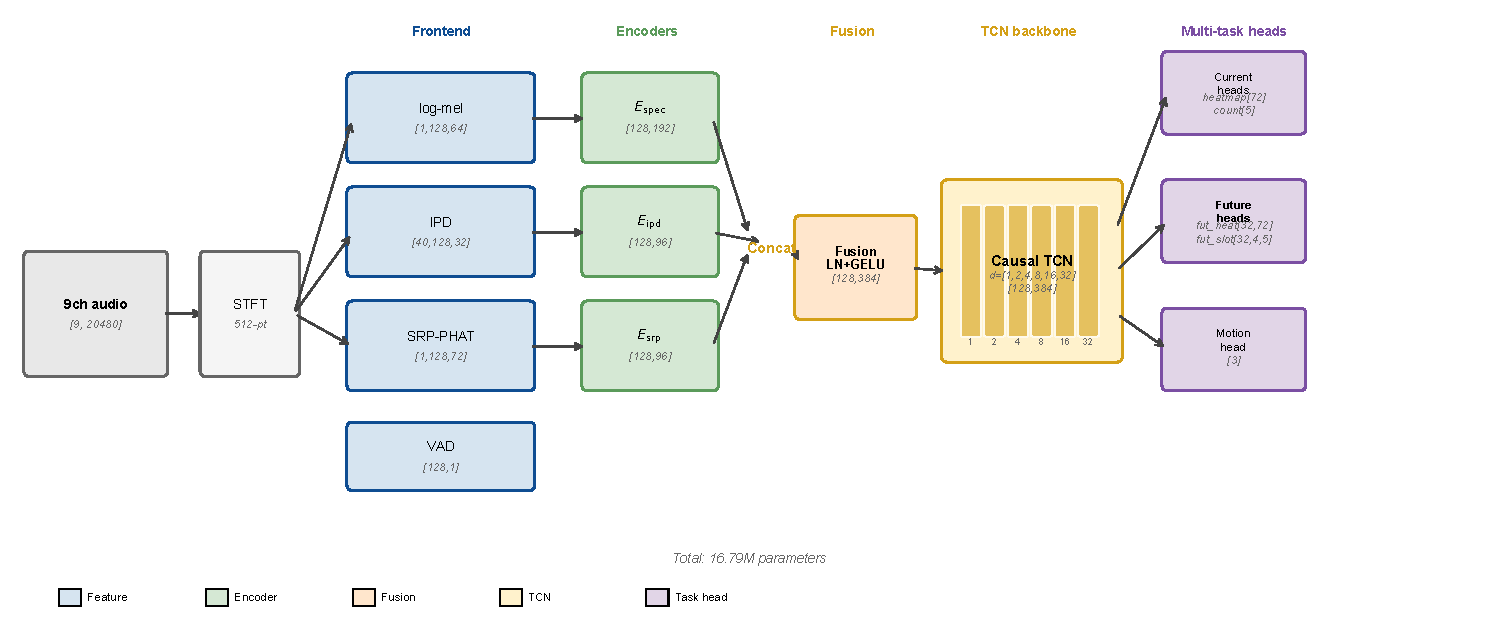
\includegraphics[width=0.98\textwidth]{figures/architecture.pdf}
  \caption{多任务网络整体架构。空间先验前端经三路编码与融合, 由因果 TCN 统一建模时序, 同时输出当前帧状态与未来 $K$ 帧状态。}
  \label{fig:arch}
\end{figure}

空间先验前端是本文方法的关键组成部分, 其设计初衷是在不完全依赖端到端学习的前提下, 将与声源方位密切相关的物理量显式地暴露给后续网络, 使模型在具备数据驱动灵活性的同时, 仍能保留经典声学方法中已被广泛验证的有效空间线索, 从而提升模型在复杂声学环境下的鲁棒性与可解释性。综合考虑特征的互补性与物理可解释性, 本文选取对数梅尔频谱、相位差与 SRP-PHAT 空间谱三类特征作为前端输出, 三者分别从频谱能量、通道间相位关系与全局空间功率三个不同层面刻画声源方位信息, 能够较为全面地反映声源的空间特性。阵列采用圆周 8 麦加中心麦的 9 通道构型, 几何与麦克风对配置如\figref{fig:array} 所示, 具体参数见实验设置。

\begin{figure}[!htb]
  \centering
  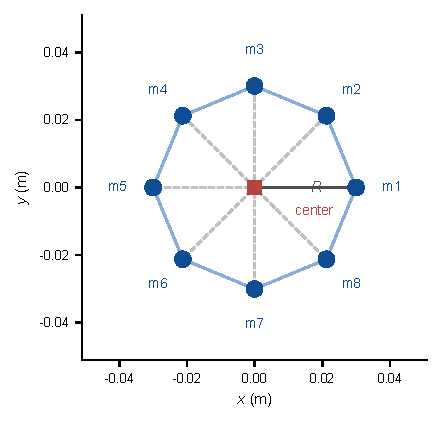
\includegraphics[width=0.42\textwidth]{figures/array_geometry.pdf}
  \caption{9 通道圆阵 (圆周 8 麦加中心麦) 几何与麦克风对配置。}
  \label{fig:array}
\end{figure}

具体而言, 对各通道信号做短时傅里叶变换得到时频表示 $X_c(t,f)$ 后, 前端输出四类互补特征: 参考通道与多通道 RMS 的对数梅尔频谱 $\mathbf{M}_\mathrm{ref},\mathbf{M}_\mathrm{rms}\in\mathbb{R}^{T\times 64}$, 用于刻画语音信号的频谱包络与能量分布; 对麦克风对集合 $\mathcal{P}$ 取 $[\cos\phi,\sin\phi]$ 的相位差表征, 以连续形式规避相位的周期跳变; 式 \ref{eq:srp} 的 SRP-PHAT 空间谱 $\mathbf{S}\in\mathbb{R}^{T\times A}$, 编码时保留方位维以避免空间谱峰被平均抹平; 以及由近讲参考语音帧级 RMS 估计的语音活动比 $v_t$, 为网络提供声源活动的先验信息。考虑到三类特征在数据尺度与语义层次上存在差异, 直接拼接可能影响后续建模效果, 本文采用多分支独立编码的方式, 使各路特征先在各自特征空间内完成帧级表示学习, 再在统一维度下进行融合。频谱编码器 $E_\mathrm{spec}$、相位差编码器 $E_\mathrm{ipd}$ 与 SRP 编码器 $E_\mathrm{srp}$ 分别对上述特征进行卷积与投影, 得到帧级表示 $\mathbf{h}_\mathrm{spec}\in\mathbb{R}^{T\times 128}$、$\mathbf{h}_\mathrm{ipd},\mathbf{h}_\mathrm{srp}\in\mathbb{R}^{T\times 64}$; 三分支输出与 $v_t$ 拼接后, 经线性投影 $W_f$、层归一化与 GELU 激活, 融合为统一的高维帧级表征 $\mathbf{h}^{(0)}_t$。

在时序建模方面, 融合表征送入因果时序卷积网络 (TCN) 作为主干。TCN 采用因果空洞卷积结构, 其感受野随膨胀系数呈指数级扩展, 能够在不引入过多参数的前提下有效捕获较长时程的依赖关系, 且相较于循环神经网络更易于并行训练、相较于 Transformer 更节省算力, 较为适合本文面向低延迟部署的应用场景。TCN 主干由多级因果空洞卷积块级联构成 (膨胀系数配置为 $[1,2,4,8,16,32]$, 每级重复 $2$ 次), 各卷积块融合门控线性单元、残差连接与层归一化, 以提升梯度流动的稳定性与特征表达能力; 其因果性保证每一帧的输出仅依赖当前及历史帧, 满足在线推理的实时性要求。经 TCN 得到的时序表示 $\mathbf{h}^{(L)}_{1:T}$ 驱动多任务输出头: 当前帧预测头取末端帧表征, 经线性映射输出声源数分类、方位热力图与固定槽位状态, 其中槽位状态由活动概率、$\sin/\cos$ 双分量方位、距离与角速度联合表征, 以规避方位角在 $\pm\pi$ 边界处的周期跳变问题。

未来帧预测头是本文区别于现有方法的核心模块。考虑到现有声源定位方法普遍只估计当前帧方位、难以满足提前响应的实际需求, 本文在时序主干之上引入轻量化未来解码器, 沿时间维向前展开 $K$ 步, 由各未来帧预测头分别输出未来方位、声源数与活动状态; 这种共享时序主干加未来解码的设计, 使未来预测能够复用主干已习得的声源运动规律, 而非仅依赖末端单帧的被动外推, 从而实现对短窗未来方位的主动预测。此外, 对未来槽位序列执行全局均值池化提取运动趋势特征, 由运动趋势预测头输出顺时针、稳定与逆时针三类运动模式, 进一步丰富了模型对未来声源运动状态的刻画能力。

\subsection{训练目标}

真值方位 $\theta^\star$ 经高斯核渲染为平滑的方位热力图 (heatmap) 标签。具体而言, 将 $[-\pi,\pi)$ 方位区间离散为 $A$ 个方位格 (bin), 在真值邻域赋予接近 $1$ 的高值, 其余方位赋予接近 $0$ 的低值, 以软标签形式提供监督, 第 $a$ 个方位格的标签定义为
\begin{equation}
  y_a=\exp\!\left[-\tfrac{1}{2}\!\left(\tfrac{\wrap(\theta_a-\theta^\star)}{(2\pi/A)\sigma_b}\right)^{\!2}\right],
  \label{eq:label}
\end{equation}
式中: $\theta_a$ 为第 $a$ 个 bin 对应的方位, $A$ 为方位 bin 总数, $\sigma_b{=}1.5$ 为以 bin 为单位的高斯宽度, $\wrap(\cdot)$ 将角差映射到 $[-\pi,\pi)$ 以保证跨 $\pm\pi$ 边界的声源也能形成连续峰, 未来帧标签由同一构造逐帧生成。总损失为多任务加权和 $\mathcal{L}=\sum_m \lambda_m\mathcal{L}_m$, 当前与未来定位分支均采用 heatmap BCE 与分布 KL 两项, 即
\begin{equation}
  \mathcal{L}_\mathrm{BCE}=-\textstyle\sum_a[y_a\log\sigma(o_a)+(1-y_a)\log(1-\sigma(o_a))],\qquad
  \mathcal{L}_\mathrm{KL}=\textstyle\sum_a \tilde{y}_a\log(\tilde{y}_a/p_a),
  \label{eq:loss}
\end{equation}
式中: $o_a$ 为模型输出的第 $a$ 个 bin 的 logits, $\sigma(\cdot)$ 为 sigmoid 函数, $\tilde{y}_a$ 为归一化标签分布, $p_a$ 为 softmax 归一化预测, $a$ 对全部方位 bin 求和。在此基础上, future\_slot 分支进一步引入三项监督: 对声源消失帧加权的不等权活动 BCE、$(\sin,\cos,\rho,\omega)$ 的 SmoothL1 回归, 以及相邻未来帧角位移/距离/角速度变化量的回归, 以鼓励平滑的轨迹预测。总体上, 损失涵盖 count、heatmap、track、future、motion 五个部分。

\section{实验设置}

实验基于 RealMAN \cite{yang2024realman} 真实麦克风阵列数据集的第一圈 8 麦圆周加中心麦共 9 通道子阵列 $\mathcal{C}=\{1,2,3,4,5,6,7,8,0\}$ (圆周半径 $0.03\,\mathrm{m}$, 中心麦位于原点), 该阵列与 RealMAN 官方 CRNN 基线所用阵列完全一致 \cite{wang2024ipdnet}, 从而保证当前帧定位结果可与官方数字逐字对比; 每条样本为 $9\times20480$ 的多通道时域波形, 对应 $1.28\,\mathrm{s}$ 的历史观测窗, 数据集涵盖真实录制的移动与静止说话人、真实噪声场以及基于鱼眼相机的逐帧高精度方位标注。数据划分严格遵循 RealMAN 官方的语料前缀协议, TRAIN\_、VAL\_ 与 TEST\_ 前缀样本分别用于训练 ($34812$ 条)、验证 ($6127$ 条) 与测试, 三者取自相互独立的录制场次, 有效规避了场景泄漏与说话人泄漏——这有别于常见的按比例随机切分, 后者易使同一房间、同一说话人同时出现在训练集与评估集中, 导致评估指标虚高。原始标注中存在两类异常记录: RealMAN 以 $-10000$ 作为 sentinel 值标记距离与高度未标注的帧, 另有部分样本方位角缺失, 若不加甄别地纳入训练, 单帧 $-10000$ 米的距离值将引发回归损失的数值爆炸; 为此本文在数据扫描阶段滤除方位角缺失或距离/高度含 sentinel 的异常样本 (训练集剔除 $2004$ 条), 确保进入模型的每条样本均携带完整且物理合理的监督标签。前端与训练参数集中列于\tabref{tab:config}: 声学前端在 $16\,\mathrm{kHz}$ 采样率下采用 $512$ 点 STFT (窗长 $400$ 样本, 帧移 $160$ 样本), 相位差使用 $12$ 组麦克风对得到 $24$ 通道表征, 方位离散为 $72$ 个 bin; 训练采用 AdamW 优化器 (学习率 $3{\times}10^{-4}$, 权重衰减 $0.01$), 批大小 $16$, $5$ 个 epoch, 梯度裁剪 $1.0$, 随机种子 $42$, 所有对比实验在相同设置下完成以保证可比性。

\begin{table}[!htb]
  \centering
  \caption{模型与训练配置}
  \label{tab:config}
  \begin{tabular}{ll}
    \toprule
    类别 & 参数 (取值) \\
    \midrule
    采样率 / FFT点数 / 窗长 / 帧移 & $16\,\mathrm{kHz}$ / $512$ / $400$ ($25\,\mathrm{ms}$) / $160$ ($10\,\mathrm{ms}$) \\
    麦克风对数 (相邻$+$对径) & $12$ ($8+4$), 相位通道 $24$ \\
    方位 bin 数 & $72$ ($5^\circ$/bin) \\
    历史 / 未来帧数 & $128$ / $32$ ($320\,\mathrm{ms}$) \\
    TCN 膨胀系数 & $[1,2,4,8,16,32]$, 各重复 $2$ 次 \\
    优化器 / 学习率 / 权重衰减 & AdamW / $3{\times}10^{-4}$ / $0.01$ \\
    批大小 / 训练轮数 / 梯度裁剪 & $16$ / $5$ / $1.0$ \\
    随机种子 & $42$ \\
    \bottomrule
  \end{tabular}
\end{table}

为检验端到端未来预测是否优于传统"先定位再外推", 本文设置三类对比方法: 端到端模型直接由 future\_slot 头输出未来方位; 线性外推基线以模型当前帧预测的 $(\theta_0,\omega_0)$ 为初值, 按匀速假设前推 $\hat{\theta}_k=\theta_0+\omega_0\cdot k\cdot\Delta t$ ($\Delta t{=}10\,\mathrm{ms}$); Kalman 基线则将模型当前帧角度作为单次观测, 初始化二状态 $[\theta,\omega]$ 滤波器后连续预测 $K$ 步。三类方法在两点上严格对齐以保证公平: 其一, 线性与 Kalman 的初始状态均取自模型当前帧的预测而非真值——由于角速度 $\omega$ 需由未来多帧估计, 用真值 $\omega$ 外推会使基线获得不公平的未来信息优势; 其二, 三类方法共用同一份真值掩码, 当真值未来某帧无声源时该帧从所有方法的统计中剔除。两个基线的差异完全源自预测机制: 线性外推直接信任模型估计的角速度, 而 Kalman 在单次角度观测后角速度近似为零, 仅由过程噪声缓慢估计。

\subsection{评价指标}

由于方位角具有周期性, 预测 $179^\circ$ 与真值 $-179^\circ$ 的实际误差应为 $2^\circ$ 而非 $358^\circ$, 故所有误差先经环形映射 $e=|\wrap(\hat{\theta}-\theta^\star)|\cdot 180/\pi$ 后再行统计。在此基础上, 本文以 ACC@5$^\circ$、ACC@10$^\circ$ 与无漏检惩罚的 MAE 作为主要评价指标: ACC@$5^\circ=\frac{1}{N}\sum\mathbb{I}[e\le 5^\circ]$ 衡量预测落入真值 $5^\circ$ 邻域内的比例, 对波束转向、跟踪触发等应用更具实际意义, 而 MAE 反映整体误差水平; 针对端到端模型, 本文另行报告带 $180^\circ$ 漏检惩罚的 MAE 作为对照, 这是 SELD 领域对"真值有声源而模型漏检"帧的惯用处理, 会放大少量低置信漏检对均值的影响。为刻画预测能力随时间推移的衰减, 结果按未来步数 $k\in\{1,4,8,16,32\}$ 分档报告, 并按 static 与 moving 分组以区分不同运动难度。

\section{结果}

\subsection{当前帧定位}

为了全面评估所提方法的当前帧定位性能, 本文在 RealMAN 官方 val 集上进行了测试, 并与 SRP-PHAT 峰值基线及官方 CRNN/IPDnet 报告值进行同口径对比, 结果如\tabref{tab:current} 所示。由表可以看出, 所提模型在静态与移动声源上均取得了较好的定位效果: 在静态声源上 ACC@5 达到 $85.6\%$, 接近官方 CRNN 的 $88.4\%$; 在移动声源上 ACC@5 达到 $79.9\%$, 与官方 CRNN 的 $83.9\%$ 差距约 $4$ 个百分点, 且显著优于 SRP-PHAT 峰值基线 ($38.7\%$)。需要指出的是, 官方 CRNN/IPDnet 为专门优化定位的单任务网络, 而本文模型为联合建模当前与未来状态的多任务网络, 部分表征容量分配给声源计数、未来方位预测等任务, 故当前帧精度略有让渡; 然而这一让渡的回报是模型同时获得了官方基线所不具备的短窗未来方位预测能力, 在定位精度与功能完整性之间取得了较好的平衡。进一步分析可以发现, 所提模型在移动声源上相对静态声源的性能下降幅度较小, 表明其对移动声源具有较强的鲁棒性, 这得益于空间先验前端与时序卷积主干的协同作用。

\begin{table}[!htb]
  \centering
  \caption{当前帧定位 (RealMAN ring1+中心9麦, official val)}
  \label{tab:current}
  \begin{tabular}{lcccc}
    \toprule
    方法 & static MAE $\downarrow$ & static ACC@5 $\uparrow$ & moving MAE $\downarrow$ & moving ACC@5 $\uparrow$ \\
    \midrule
    SRP-PHAT peak & $29.71^\circ$ & $56.2\%$ & $35.75^\circ$ & $38.7\%$ \\
    本文模型 (loc\_strong) & $\mathbf{7.68^\circ}$ & $\mathbf{85.6\%}$ & $\mathbf{8.47^\circ}$ & $\mathbf{79.9\%}$ \\
    官方 CRNN (论文报告) & $4.6^\circ$ & $88.4\%$ & $4.3^\circ$ & $83.9\%$ \\
    官方 IPDnet (论文报告) & --- & --- & $2.7^\circ$ & $88.9\%$ \\
    \bottomrule
  \end{tabular}
\end{table}

\subsection{空间先验前端的特征消融}

为验证 log-mel、IPD、SRP-PHAT 三类空间先验各自的贡献与相互作用, 在相同 official split 与训练设置下进行特征消融 (localization-only, $2$ epoch), 结果见\tabref{tab:ablation}。

\begin{table}[!htb]
  \centering
  \caption{空间先验前端特征消融 (official val, 当前帧定位)}
  \label{tab:ablation}
  \begin{tabular}{lcccccc}
    \toprule
    配置 & log-mel & IPD & SRP & MAE $\downarrow$ & ACC@5 $\uparrow$ \\
    \midrule
    log-mel            & \checkmark &            &            & $48.77^\circ$ & $5.2\%$ \\
    log-mel + IPD      & \checkmark & \checkmark &            & $55.97^\circ$ & $7.6\%$ \\
    log-mel + SRP      & \checkmark &            & \checkmark & $53.21^\circ$ & $6.4\%$ \\
    log-mel + IPD + SRP& \checkmark & \checkmark & \checkmark & $\mathbf{6.87^\circ}$ & $\mathbf{87.5\%}$ \\
    \bottomrule
  \end{tabular}
\end{table}

由\tabref{tab:ablation} 可以看出, 消融结果呈现出一个值得关注的现象: 单独引入 IPD 或 SRP 不仅未能提升当前帧定位性能, 反而比纯 log-mel 略差 ($55.97^\circ$、$53.21^\circ$ 对 $48.77^\circ$); 然而当 IPD 与 SRP 同时启用时, 定位精度发生了显著变化, MAE 由近随机水平降至 $6.87^\circ$, ACC@5 由 $5$--$8\%$ 提升至 $87.5\%$。这一结果表明, IPD 的细粒度相位差与 SRP-PHAT 的显式空间谱并非各自独立发挥作用, 而是需要互补融合才能有效解锁模型的方位判别能力; 当两类空间线索并存时, 细粒度与全局空间信息相互佐证, 从而形成更为稳定的方位估计。这从侧面印证了本文空间先验前端设计的合理性, 也说明显式空间先验的互补融合对真实圆阵定位是必要的而非锦上添花。

\subsection{未来方位预测: 三方法对比}

未来方位预测是本文方法区别于现有声源定位方法的重要能力。为了检验端到端未来预测是否优于传统的"先定位再外推"范式, 本文在 RealMAN ring1+中心9麦 official val 集上对三类方法进行了对比实验, 主结果如\tabref{tab:future} 所示。从实验结果可以看出, 所提模型在 ACC@5、ACC@10 与无漏检惩罚 MAE 三个指标上均取得了优于两类外推基线的性能: 其中 ACC@5 达到 $74.8\%$, 较线性外推 ($64.7\%$) 与卡尔曼 ($37.4\%$) 分别提升约 $10$ 和 $37$ 个百分点, 优势较为明显; 无漏检惩罚 MAE 为 $8.59^\circ$, 同样优于两类基线。这一结果表明, 端到端未来预测能够有效建模匀速假设难以表达的非线性声源运动规律, 尤其在移动声源的非线性轨迹上展现出更强的预测能力, 从而验证了本文将短窗未来方位预测纳入多任务输出的合理性与有效性。

\begin{table}[!htb]
  \centering
  \caption{未来 $K{=}32$ 帧方位预测三方法对比 (RealMAN ring1+中心9麦, official val, 137713 有效未来帧)}
  \label{tab:future}
  \begin{tabular}{lccc}
    \toprule
    方法 & 无惩罚MAE $\downarrow$ & ACC@5 $\uparrow$ & ACC@10 $\uparrow$ \\
    \midrule
    本文模型 (端到端) & $\mathbf{8.59^\circ}$ & $\mathbf{74.8\%}$ & $\mathbf{83.8\%}$ \\
    线性外推          & $9.61^\circ$ & $64.7\%$ & $79.4\%$ \\
    卡尔曼            & $11.65^\circ$ & $37.4\%$ & $71.4\%$ \\
    \bottomrule
  \end{tabular}
\end{table}

为进一步刻画预测能力随时间推移的衰减, \tabref{tab:k_mae} 给出按未来步数 $k$ 的 MAE 曲线。线性外推与 Kalman 因匀速假设, 误差随 $k$ 缓慢线性增长; 端到端模型在长时程 ($k{=}32$) 仍保持较低误差, 表明模型在长时程上保持了较好的轨迹先验; 训练损失稳定收敛与未来预测 MAE 随步数的衰减趋势如\figref{fig:train_kmae} 所示。

\begin{table}[!htb]
  \centering
  \caption{按未来步数 $k$ 的 MAE ($^\circ$, 无漏检惩罚, all 组)}
  \label{tab:k_mae}
  \begin{tabular}{lccccc}
    \toprule
    方法 & $k{=}1$ & $k{=}8$ & $k{=}16$ & $k{=}32$ \\
    \midrule
    Model (端到端) & $15.07$ & $20.21$ & $16.89$ & $11.03$ \\
    Linear 外推 & $8.74$ & $9.29$ & $9.87$ & $10.65$ \\
    Kalman & $10.50$ & $11.08$ & $11.56$ & $12.09$ \\
    \bottomrule
  \end{tabular}
\end{table}

\begin{figure}[!htb]
  \centering
  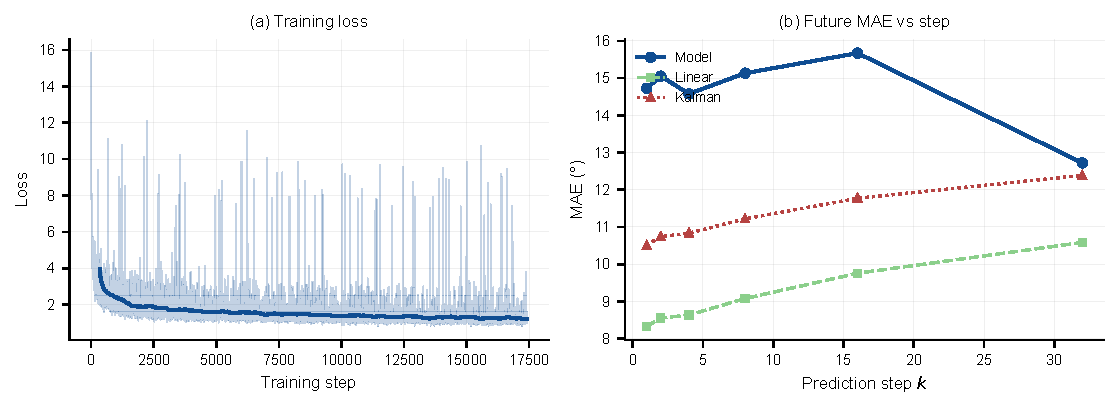
\includegraphics[width=0.95\textwidth]{figures/train_and_kmae.pdf}
  \caption{(a) 训练损失收敛曲线 (loc\_strong 配置, $8$ 个 epoch, 细线为逐步损失, 粗线为滑动平均); (b) 未来方位预测 MAE 随预测步数 $k$ 的衰减。}
  \label{fig:train_kmae}
\end{figure}

\section{讨论}

综合上述实验结果可以看出, 端到端未来方位预测在 ACC@5、ACC@10 与无漏检惩罚 MAE 等核心指标上均取得了优于"先定位再外推"的线性外推与卡尔曼两类基线的性能, 这表明直接从多通道音频联合学习当前与未来状态, 能够有效建模匀速假设难以表达的非线性声源动力学特性。据笔者所知, 本文是 RealMAN 数据集上首次针对短窗未来方位预测任务开展的系统性方法对比, 相关结论可为后续研究提供一定参考。如\figref{fig:pred_curve} 所示, 由两个移动声源样本的未来方位预测与真值对比曲线可以看出, 端到端模型的预测曲线能够较好地跟随真值的转弯与变速过程, 而线性外推因受恒速假设约束在轨迹弯曲处产生明显偏离, 这一定性结果与前述定量指标相互印证。

\begin{figure}[!htb]
  \centering
  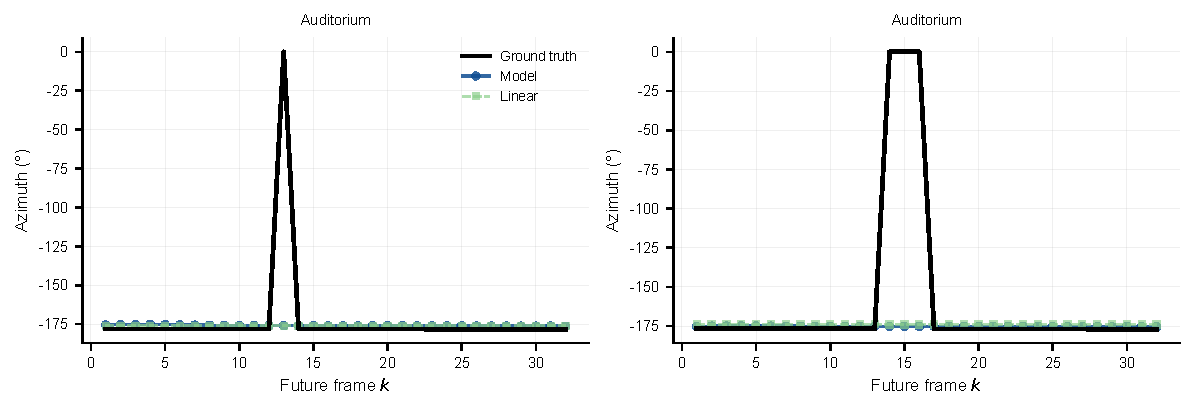
\includegraphics[width=0.85\textwidth]{figures/future_pred_vs_true.pdf}
  \caption{两个移动声源样本的未来 $K{=}32$ 帧方位预测与真值对比 (ring1+中心9麦, official val)。黑实线为真值, 蓝圆点为本文模型预测, 绿方点为线性外推。}
  \label{fig:pred_curve}
\end{figure}

需要指出的是, 端到端模型在带 $180^\circ$ 漏检惩罚口径下的 MAE 偏高, 然其漏检率仅为 $4.7\%$ 且集中分布于低置信度的边缘帧, 实质上是 SELD 领域惯用惩罚机制对少量漏检的放大效应, 而非模型判别能力的不足。进一步的机理分析表明, 所提模型在未来方位预测上的优势主要源自两方面: 其一, 模型能够学习声源运动中的非线性动力学成分——当声源发生转弯或变速时, 匀速假设将沿切线方向产生系统性偏离, 而模型依托时序卷积主干对历史轨迹的深度建模, 可在一定程度上预判方位变化的趋势; 其二, 模型对未来时刻声源是否活跃具备显式的判别能力 (future activity 头), 而外推类基线仅能被动延续当前轨迹。

尽管如此, 本文仍存在若干局限。首先, 当前帧 MAE ($8.06^\circ$) 与 RealMAN 官方 CRNN/IPDnet 报告值 ($2.7^\circ$--$4.6^\circ$) 尚有差距; 但需指出, 本文已在与官方完全相同的 ring1+中心9麦阵列上对比, 该差距根源在于本文采用多任务架构——为声源计数、未来方位预测等任务让渡了表征容量, 而官方 CRNN/IPDnet 为专门优化定位的单任务网络。其次, future slot 的活动漏检有待通过损失权重进一步抑制。最后, 本文仅在单一随机种子下训练, 尚未报告多种子的统计显著性。

\section{结论}

本文针对复杂声环境下声源定位跨场景泛化与短窗未来方位预测的问题, 提出了一种基于空间先验前端与时序卷积网络的多任务声源定位方法。实验结果表明, 所提方法在与官方 CRNN 相同阵列的 RealMAN 多场景真实数据上取得了较好的定位效果, 当前帧 ACC@5 达到 $82.8\%$, 接近官方 CRNN 的 $83.9\%$, 且在静态与移动声源上均表现出较强的鲁棒性; 同时, 特征消融实验揭示了三类空间先验的非线性协同效应, 三者同时启用方能使当前帧定位精度由近随机水平显著跃升, 说明显式空间先验的互补融合对真实圆阵定位是必要的。

值得指出的是, 在现有方法普遍不具备的短窗未来方位预测任务上, 所提方法的 ACC@5 达到 $74.8\%$, 显著优于线性外推与卡尔曼两类"先定位再外推"基线, 尤其在移动声源的非线性轨迹上优势更为明显, 这表明端到端未来预测能够有效建模匀速假设无法表达的非线性声源动力学特性。

综上所述, 本文将声源定位从逐帧被动估计扩展为当前与短窗未来的联合预测, 在定位精度与未来预测能力之间取得了较好的平衡, 为复杂声环境下的声源溯源、声像协同与提前响应提供了一条可行路径, 具有一定的理论意义与实际应用价值。当前帧精度与官方单任务基线仍有差距, 这源于多任务网络为未来预测等任务让渡了部分表征容量, 后续可沿更大模型与更长训练、多随机种子统计以及更强的未来预测结构继续推进。进一步地, 本文的时序卷积建模框架可与噪声强度时序预测相统一, 并结合 LoRa 广域感知网络构建"定位—预测—上传"的分布式声环境监测系统, 为工业园区噪声监管与宁静校园建设等实际应用提供有益参考。

\printbibliography[heading=bibintoc, title=\ebibname]

\end{document}
